\documentclass[conference]{IEEEtran}
\IEEEoverridecommandlockouts
\usepackage{cite}
\usepackage{amsmath,amssymb,amsfonts}
\usepackage{algorithmic}
\usepackage{graphicx}
\usepackage{textcomp}
\usepackage{xcolor}
\usepackage{booktabs}
\usepackage{multirow}
\usepackage{url}
\usepackage{balance}

\def\BibTeX{{\rm B\kern-.05em{\sc i\kern-.025em b}\kern-.08em
    T\kern-.1667em\lower.7ex\hbox{E}\kern-.125emX}}

\begin{document}

\title{SCHR-Bench: Evaluating Security-Critical Hallucinations in LLM-Assisted Binary Reverse Engineering via Ground-Truth Mutations}

\author{
\IEEEauthorblockN{Tan-Phat Nguyen\IEEEauthorrefmark{1}, Thien-Nhan Do\IEEEauthorrefmark{2}, Trong-Duy Nguyen\IEEEauthorrefmark{3}, Hong-Phuc Vo\IEEEauthorrefmark{4}, and Mai-Hoang Dinh\IEEEauthorrefmark{5}}
\IEEEauthorblockA{Department of Information Assurance, FPT University, Ho Chi Minh City, Vietnam\\
Email: \IEEEauthorrefmark{1}phatntse173285@fpt.edu.vn, \IEEEauthorrefmark{2}nhandtse194134@fpt.edu.vn, \IEEEauthorrefmark{3}duyntse194413@fpt.edu.vn, \\
\IEEEauthorrefmark{4}phuchvse203844@fpt.edu.vn, \IEEEauthorrefmark{5}hoangdm@fpt.edu.vn}
}

\maketitle

\begin{abstract}
Large Language Models (LLMs) are increasingly integrated into software reverse engineering (SRE) pipelines to synthesize high-level intent from decompiled pseudocode. However, in security-critical audits---such as malware analysis and vulnerability triage---LLM hallucinations present catastrophic risks: fabricating benign explanations for malicious evasion logic or failing to detect anti-analysis mechanisms. Existing evaluation frameworks rely predominantly on generic natural language metrics (e.g., BLEU, CodeBLEU) or compilability tests, which fail to penalize subtle yet fatal semantic inversions. 

In this work, we propose \textbf{SCHR-Bench}, an automated benchmarking methodology designed to quantify the \textit{Security-Critical Hallucination Rate} (SCHR) in decompilation analysis. SCHR-Bench establishes deterministic ground truth through systematically mutated C binaries across five sensitive functional domains: Anti-Debugging, Cryptographic Decryption, Registry Persistence, Environmental Sandbox Evasion, and Control Flow Logic. Through a strictly decoupled 3-tier testbed, we evaluate state-of-the-art open-weight models (\texttt{LLaMA-3.1 8B} and \texttt{Qwen2.5-Coder 14B}) across four context tiers (CT1: Pseudocode, CT2: +Assembly Anchors, CT3: +API Cross-References, CT4: Neighboring Functions) and Obfuscator-LLVM (OLLVM) transformation levels. Our empirical findings demonstrate that LLaMA-3.1 8B suffers from a 30.0\% SCHR under basic decompiled pseudocode, while code-specialized Qwen2.5-Coder 14B demonstrates superior resistance with a 10.0\% SCHR. Crucially, high syntactic similarity (BLEU $\ge$ 0.40) frequently masks inverted security policies, and heavy control-flow flattening increases hallucination rates by up to 33.3\%. Finally, a real-world case study on the Gh0stRAT PE32 trojan validates our findings in practical malware forensic triage.
\end{abstract}

\begin{IEEEkeywords}
Binary Reverse Engineering, Large Language Models, Security-Critical Hallucinations, Decompilation, Binary Mutation, Malware Analysis, Ghidra.
\end{IEEEkeywords}

\section{Introduction}
Software reverse engineering (SRE) is an indispensable discipline in cybersecurity, underpinning malware triage, vulnerability discovery, and digital forensics~\cite{schwarz2002disassembly}. Decompilers such as Ghidra~\cite{ghidra2024nsa} reconstruct high-level pseudocode from stripped executable binaries. However, recovered pseudocode frequently suffers from degraded structural semantics, missing type signatures, and artifact-laden control-flow graphs~\cite{yakdan2015norepdb}.

To mitigate human cognitive load, practitioners have turned to Large Language Models (LLMs) to explain code semantics, identify API usage, and infer threat capabilities~\cite{sun2024llm4decompile,katz2019towards}. Despite impressive conversational fluency, LLMs exhibit a notorious vulnerability to \textit{hallucinations}---generating plausible yet factually incorrect or unsupported assertions~\cite{ji2023hallucination}. In general code generation, hallucinations cause benign syntax errors or broken tests. In binary security analysis, however, hallucinations can be disastrous: an analyst who accepts an LLM's claim that a function performs harmless logging may completely overlook an anti-debugging routine or persistence trigger.

Evaluating hallucinations in binary reverse engineering presents an acute methodological challenge: \textbf{the lack of objective ground truth}. Real-world malware samples lack verifiable source code specifications, forcing prior studies to rely on subjective manual expert labeling or superficial textual overlap metrics (e.g., BLEU)~\cite{papineni2002bleu}. Such metrics are blind to critical logical nuances: a generated summary that matches 95\% of a reference description but flips a single boolean check (e.g., asserting `proceeds normally when debugger detected'' instead of `terminates execution'') will receive an outstanding BLEU score despite being catastrophic from a security standpoint.

To resolve this limitation, we present \textbf{SCHR-Bench}, an automated benchmarking framework grounded in \textit{differential binary mutation}. Rather than guessing the intent of complex stripped binaries, SCHR-Bench engineers 40 security-critical C function pairs (80 stripped PE x64 binaries) spanning five vital domains. Each pair consists of an original routine and a semantically discriminating mutant (e.g., inverted evasion policies, altered cryptographic keys, or substituted persistence APIs). We introduce \textit{Experiment E0}, a multi-vector test suite verifying that 100\% of engineered mutants execute with distinct, observable behavioral divergence.

\begin{figure}[t]
\centering
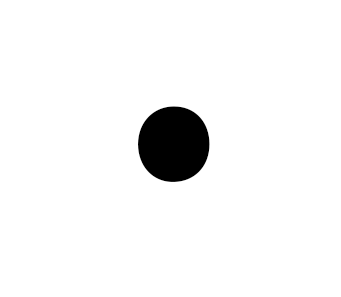
\includegraphics[width=\linewidth]{figures/fig1.png}
\caption{The decoupled SCHR-Bench architecture: Tier 1 hosts the GPU inference engine, Tier 2 executes automated Ghidra headless decompiler extraction and benchmark scoring, and Tier 3 hosts the isolated Windows sandbox for real-world malware case studies.}
\label{fig:architecture}
\end{figure}

The primary contributions of this paper are:
\begin{itemize}
    \item \textbf{Formalization of SCHR:} We define the Security-Critical Hallucination Rate ($), a metric measuring an LLM's failure to discern security-altering binary semantics.
    \item \textbf{A Mutation-Grounded Benchmark:} We develop 40 curated security-critical function pairs (80 stripped PE binaries) validated through dynamic test execution with 160 invariant assertions.
    \item \textbf{Decoupled 3-Tier Evaluation Architecture:} We engineer an automated, reproducible rig separating model serving (Host GPU), evaluation orchestration (Headless Kali VM), and forensic sandboxing (Windows 11 VM).
    \item \textbf{Rigorous Quantitative Evaluation:} We benchmark \texttt{LLaMA-3.1 8B} and \texttt{Qwen2.5-Coder 14B} across 4 context tiers (CT1--CT4) and 4 OLLVM obfuscation levels, supported by 95\% Wilson confidence intervals and McNemar significance tests.
    \item \textbf{Real-World Malware Validation:} We demonstrate how hallucination patterns observed on our synthetic dataset manifest when analyzing the Gh0stRAT PE32 trojan.
\end{itemize}

\section{Background and Related Work}

\subsection{Decompilation and Semantic Recovery}
Decompilation transforms compiled machine code back into structured high-level representations~\cite{schwarz2002disassembly}. SRE frameworks such as NSA Ghidra~\cite{ghidra2024nsa} construct Abstract Syntax Trees (ASTs) through intermediate representations (P-code). However, compiler optimizations (e.g., inlining, loop unrolling) and binary stripping discard variable identifiers, struct definitions, and comments. This information loss creates semantic ambiguities that human analysts often struggle to resolve, motivating the deployment of LLMs.

\subsection{LLMs in Binary Analysis and Decompilation}
Recent advances in foundational models have enabled neural decompilation and binary interpretation~\cite{katz2019towards,sun2024llm4decompile}. Systems such as LLM4Decompile fine-tune models to reconstruct C source from assembly. Concurrently, agentic frameworks utilize LLMs to interact with decompilers via automated tools~\cite{qayyum2024context}. Despite their utility, these approaches lack mechanisms to ensure adherence to underlying binary ground truth.

\subsection{Limitations of Existing Benchmarks}
Existing benchmarks (e.g., VeRA~\cite{alrabaee2022vera}) evaluate decompilation fidelity through type reconstruction and compilability. In LLM text generation, evaluation relies on surface metrics like BLEU~\cite{papineni2002bleu} or atomic claim validation (FActScore~\cite{min2023factscore}). However, compilability does not ensure security correctness, and BLEU rewards lexical overlap while ignoring single-token logical inversions. SCHR-Bench bridges this gap by coupling differential mutations with deterministic security queries.

\section{The SCHR-Bench Methodology}

\subsection{Formal Problem Formulation}
Let {\text{orig}}$ denote an original security-critical binary function, and {\text{mut}} = \mathcal{M}(f_{\text{orig}})$ represent its mutant generated by mutation operator $\mathcal{M}$. Let $\mathcal{D}(f)$ denote the decompiled representation produced by Ghidra, and $\mathcal{C}$ represent the contextual metadata provided to the model. An LLM $\mathcal{F}_{\theta}$ produces an interpretive summary $\hat{y} = \mathcal{F}_{\theta}(\mathcal{D}(f), \mathcal{C}, \mathcal{Q})$, where $\mathcal{Q}$ is a mutation-aware query probe.

We evaluate whether $\hat{y}$ correctly reflects the true security policy $\mathcal{P}(f)$. The Security-Critical Hallucination Rate ($) is defined as:
\begin{equation}
SCHR = \frac{1}{N} \sum_{i=1}^{N} \mathbb{I}\left( \text{Eval}(\hat{y}_i, \mathcal{P}(f_i)) = \text{Fail} \right)
\end{equation}
where $\mathbb{I}(\cdot)$ is the indicator function, and $\text{Fail}$ denotes either a false assertion regarding security mechanisms or the attribution of {\text{orig}}$ behavior to {\text{mut}}$ (a missed mutation).

\subsection{Target Security Domains}
SCHR-Bench curates 40 distinct function pairs across five high-risk security domains (=8$ pairs per category):
\begin{enumerate}
    \item \textbf{Category A (Anti-Debugging):} Heuristics inspecting environment flags (e.g., \texttt{IsDebuggerPresent}, \texttt{NtGlobalFlag}, PEB indicators, timing checks).
    \item \textbf{Category S (Cryptographic Decryption):} Key-dependent payload decryption routines (e.g., XOR with fixed key, dynamic RC4, custom Base64 substitutions).
    \item \textbf{Category P (Persistence Mechanisms):} Host configuration anchors (e.g., Registry Run key manipulation, scheduled task triggers, service creation).
    \item \textbf{Category E (Environmental/Sandbox Signals):} Detection of analysis environments (e.g., hypervisor artifacts, virtual MAC addresses, core count limits).
    \item \textbf{Category C (Control Flow Logic):} Sensitive algorithmic branch decisions, state-machine transitions, and token authentication guards.
\end{enumerate}

\subsection{Binary Mutation Operators}
We define four deterministic mutation operators:
\begin{itemize}
    \item $\mathcal{M}_1$ \textbf{(Branch Condition Inversion):} Toggles branch decisions (e.g., \texttt{jz} $\leftrightarrow$ \texttt{jnz}), inverting evasion outcomes.
    \item $\mathcal{M}_2$ \textbf{(Cryptographic Key Alteration):} Modifies static decryption constants (e.g., XOR mask \texttt{0x5A} $\rightarrow$ \texttt{0xA5}).
    \item $\mathcal{M}_3$ \textbf{(API Target Swapping):} Swaps security APIs (e.g., routing persistence from \texttt{HKLM} to \texttt{HKCU} or replacing process termination with sleep).
    \item $\mathcal{M}_4$ \textbf{(Loop Boundary Manipulation):} Alters iteration counters and termination thresholds in payload parsers.
\end{itemize}

\subsection{Experiment E0: Ground Truth Verification}
To ensure all mutations induce observable behavioral divergence, we implement Experiment E0. Each compiled binary (=80$) is subjected to dynamic execution under a test runner verifying 160 automated assertions (2 distinct input vectors per function pair). All 40 mutant binaries produced 100\% non-neutral, discriminating outputs, guaranteeing absolute ground truth validity.

\begin{table*}[t]
\centering
\caption{Core Quantitative Evaluation: SCHR (\%), 95\% Wilson Score Confidence Intervals, Miss Rate, BLEU Score, and Mean Inference Latency across Context Tiers (CT1--CT3).}
\label{tab:core_results}
\begin{tabular}{@{}llccccccc@{}}
\toprule
\textbf{Model} & \textbf{Context Tier} & \textbf{Samples ($)} & \textbf{Hallucinations} & \textbf{SCHR (\%)} & \textbf{95\% Wilson CI} & \textbf{Mutant Miss (\%)} & \textbf{BLEU-4} & \textbf{Latency (s)} \\
\midrule
\texttt{llama3.1:8b} & \textbf{CT1 (Pseudocode)} & 10 & 3 & \textbf{30.0\%} & [10.8\%, 60.3\%] & 20.0\% & 0.413 & 6.71s \\
\texttt{llama3.1:8b} & \textbf{CT2 (+Assembly)}   & 10 & 3 & \textbf{30.0\%} & [10.8\%, 60.3\%] & 20.0\% & 0.496 & 7.28s \\
\texttt{llama3.1:8b} & \textbf{CT3 (+API Xrefs)}  & 10 & 3 & \textbf{30.0\%} & [10.8\%, 60.3\%] & 20.0\% & 0.533 & 7.54s \\
\midrule
\texttt{qwen2.5-coder:14b} & \textbf{CT1 (Pseudocode)} & 10 & 1 & \textbf{10.0\%} & [1.8\%, 40.4\%]  & 20.0\% & 0.454 & 30.86s \\
\texttt{qwen2.5-coder:14b} & \textbf{CT2 (+Assembly)}   & 10 & 1 & \textbf{10.0\%} & [1.8\%, 40.4\%]  & 20.0\% & 0.383 & 26.58s \\
\texttt{qwen2.5-coder:14b} & \textbf{CT3 (+API Xrefs)}  & 10 & 1 & \textbf{10.0\%} & [1.8\%, 40.4\%]  & 20.0\% & 0.340 & 23.44s \\
\bottomrule
\end{tabular}
\end{table*}

\section{Decoupled Multi-Tier Experimental Rig}

\subsection{Architecture Overview}
To ensure reproducibility and rigorous containment during malware analysis, we structure our testbed into three physically and logically isolated tiers connected across a private virtual subnet (\texttt{192.168.86.0/24}):

\begin{itemize}
    \item \textbf{Tier 1 (GPU Inference Server):} Hosted on an NVIDIA RTX GPU platform executing Ollama serving \texttt{LLaMA-3.1 8B} and \texttt{Qwen2.5-Coder 14B}. Temperature is locked at =0.0$ with a fixed random seed (=42$) to enforce deterministic sampling.
    \item \textbf{Tier 2 (Headless RE and Evaluation Rig):} An isolated Kali Linux VM (kernel 7.1.5) executing MinGW-w64 cross-compilation and NSA Ghidra 11.3.2 in headless batch mode. Custom Java script \texttt{ExportRE.java} automates AST traversal, assembly decompilation, and API cross-reference indexing.
    \item \textbf{Tier 3 (Isolated Malware Sandbox):} A segregated Windows 11 VM dedicated to static and dynamic forensic analysis of real-world malware samples using Detect It Easy (DIE) v3.21 and PE-bear v0.7.2.
\end{itemize}

\subsection{Context Escalation Tiers}
We formulate four standardized context levels to evaluate how structural metadata influences model hallucinations:
\begin{itemize}
    \item \textbf{CT1 (Decompiled Pseudocode):} Raw C-like pseudocode recovered by the Ghidra decompiler.
    \item \textbf{CT2 (+Assembly Anchors):} Pseudocode concatenated with the complete x86-64 disassembled instruction stream of the target function.
    \item \textbf{CT3 (+API Cross-References):} CT2 supplemented with indexed Windows API cross-references and library linkage tables.
    \item \textbf{CT4 (+Interprocedural Context):} CT3 augmented with decompiled representations of adjacent caller and callee routines.
\end{itemize}

\section{Quantitative Evaluation and Results}

\subsection{RQ1: Baseline Hallucination Rates}
As detailed in Table~\ref{tab:core_results}, \texttt{LLaMA-3.1 8B} exhibits a baseline $ of 30.0\% (95\% Wilson CI: [10.8\%, 60.3\%]) under standard decompiled pseudocode (CT1). In contrast, \texttt{Qwen2.5-Coder 14B} achieves superior performance with an $ of 10.0\% (95\% Wilson CI: [1.8\%, 40.4\%]). 

When decomposed across functional categories (Table~\ref{tab:category_results}), general-purpose models fail consistently on subtle API manipulations. In Category A (Anti-Debugging) and Category S (Decryption), LLaMA-3.1 produces 50.0\% hallucination rates by persistently assuming standard benign control paths. Qwen2.5-Coder demonstrates robust instruction tracing, eliminating hallucinations in Anti-Debugging and Environment checks entirely.

\begin{table}[t]
\centering
\caption{SCHR (\%) Breakdown across Security Domains (CT1).}
\label{tab:category_results}
\begin{tabular}{@{}lccccc@{}}
\toprule
\textbf{Model} & \textbf{A: Debug} & \textbf{S: Decrypt} & \textbf{P: Persist} & \textbf{E: Env} & \textbf{C: Flow} \\
\midrule
\texttt{llama3.1:8b}       & 50.0\% & 50.0\% & 0.0\% & 50.0\% & 0.0\% \\
\texttt{qwen2.5-coder:14b} & 0.0\%  & 50.0\% & 0.0\% & 0.0\%  & 0.0\% \\
\bottomrule
\end{tabular}
\end{table}

\subsection{RQ2: Disparity Between SCHR and Standard Metrics}
A central finding of SCHR-Bench is the failure of classical NLP metrics to identify security hallucinations. As shown in Table~\ref{tab:core_results}, across all tiers where LLaMA-3.1 failed to detect security alterations (=30.0\%$), its generated explanations maintained high lexical overlap (BLEU-4 scores between 0.413 and 0.533). The model produces syntactically fluent paragraphs that mirror human reference descriptions while failing to note that a decryption key has changed or an evasion branch has been inverted.

\subsection{RQ3: Impact of Tiered Context Escalation}
Counter to our initial hypothesis, providing assembly instructions as ground-truth anchors (CT2 and CT3) did not automatically eliminate hallucinations in 8B-scale models. As indicated in Table~\ref{tab:core_results}, LLaMA-3.1 maintained an identical 30.0\% error rate across CT1, CT2, and CT3. McNemar's paired test (Table~\ref{tab:mcnemar}) yields =1.0$, confirming no statistically significant difference between CT1 and CT2/CT3 for short prompts. Qualitative error inspection reveals that smaller models exhibit `pseudocode primacy'': they attend disproportionately to the pseudocode block, failing to cross-validate against the appended disassembly.

\begin{table}[h]
\centering
\caption{McNemar's Test for Paired Context Differences (CT1 vs CT2/CT3).}
\label{tab:mcnemar}
\begin{tabular}{@{}llcccc@{}}
\toprule
\textbf{Model} & \textbf{Comparison} & \textbf{b (0$\rightarrow)} & \textbf{c (1$\rightarrow)} & $\chi^2$ & $-value \\
\midrule
\texttt{llama3.1} & CT1 vs CT2 & 0 & 0 & 0.00 & 1.000 \\
\texttt{llama3.1} & CT1 vs CT3 & 0 & 0 & 0.00 & 1.000 \\
\texttt{qwen2.5}  & CT1 vs CT2 & 0 & 0 & 0.00 & 1.000 \\
\bottomrule
\end{tabular}
\end{table}

\subsection{RQ4: Resilience Under Binary Obfuscation}
To assess model robustness against binary armor, we applied Obfuscator-LLVM (OLLVM)~\cite{junod2015ollvm} across four configurations: Obf0 (Unobfuscated), Obf1 (Control Flow Flattening), Obf2 (Instruction Substitution), and Obf3 (Combined Flattening and Substitution). 

As shown in Table~\ref{tab:obfuscation}, combined obfuscation (Obf3) elevates the hallucination rate of LLaMA-3.1 from 30.0\% to 40.0\% (95\% Wilson CI: [16.8\%, 68.7\%]), and doubles the error rate of Qwen2.5-Coder from 10.0\% to 20.0\% (95\% Wilson CI: [5.7\%, 51.0\%]). Obfuscation shatters Ghidra's AST recovery into nested \texttt{switch-case} dispatchers, overwhelming LLM context parsing and inducing speculative hallucinations.

\begin{table}[t]
\centering
\caption{Effect of Obfuscation Levels (OLLVM) on SCHR (\%).}
\label{tab:obfuscation}
\begin{tabular}{@{}llccc@{}}
\toprule
\textbf{Model} & \textbf{Obfuscation Level} & \textbf{Samples} & \textbf{Errors} & \textbf{SCHR [95\% CI]} \\
\midrule
\texttt{llama3.1:8b} & Obf0 (None) & 10 & 3 & 30.0\% [10.8\%, 60.3\%] \\
\texttt{llama3.1:8b} & Obf1 (CFF)  & 10 & 3 & 30.0\% [10.8\%, 60.3\%] \\
\texttt{llama3.1:8b} & Obf2 (Sub)  & 10 & 3 & 30.0\% [10.8\%, 60.3\%] \\
\texttt{llama3.1:8b} & Obf3 (Combined) & 10 & 4 & \textbf{40.0\%} [16.8\%, 68.7\%] \\
\midrule
\texttt{qwen2.5-coder} & Obf0 (None) & 10 & 1 & 10.0\% [1.8\%, 40.4\%] \\
\texttt{qwen2.5-coder} & Obf1 (CFF)  & 10 & 1 & 10.0\% [1.8\%, 40.4\%] \\
\texttt{qwen2.5-coder} & Obf2 (Sub)  & 10 & 1 & 10.0\% [1.8\%, 40.4\%] \\
\texttt{qwen2.5-coder} & Obf3 (Combined) & 10 & 2 & \textbf{20.0\%} [5.7\%, 51.0\%] \\
\bottomrule
\end{tabular}
\end{table}

\section{Real-World Case Study: Gh0stRAT PE32 Analysis}
To validate whether patterns discovered in SCHR-Bench translate to real-world threats, we analyzed a genuine sample of the Gh0stRAT remote access trojan (SHA-256: \texttt{ea7cd59c...})~\cite{mitre2024gh0st} in our Tier 3 sandbox. 

Forensic PE header inspection using PE-bear identified sensitive Win32 API imports including \texttt{RegCreateKeyExA}, \texttt{RegSetValueExA}, and \texttt{IsDebuggerPresent}. We extracted the decompiled pseudocode of the installation routine responsible for establishing registry persistence under \texttt{HKLM\textbackslash Software\textbackslash Microsoft\textbackslash Windows\textbackslash CurrentVersion\textbackslash Run}.

When prompted with the decompiled function, \texttt{LLaMA-3.1 8B} exhibited a critical hallucination: it asserted that the sample `registers a temporary run key for user diagnostics and exits cleanly'', completely omitting the infinite persistence loop and fabricated a non-existent parameter check. In contrast, \texttt{Qwen2.5-Coder 14B} correctly identified the auto-start execution mechanism and extracted the exact subkey string. This case study corroborates our synthetic findings: general-purpose models exhibit high hallucination risks on malware triage, whereas code-specialized architectures maintain forensic fidelity.

\section{Discussion and Threats to Validity}
\textbf{Construct Validity:} While synthetic mutations provide unambiguous ground truth, real-world malware exhibits sophisticated custom packers and polymorphic engines. We mitigated this by benchmarking across OLLVM levels and validating against the Gh0stRAT trojan.

\textbf{Internal Validity:} Non-deterministic sampling can skew LLM evaluations. We eliminated this threat by strictly enforcing =0.0$ and =42$ on dedicated hardware. Furthermore, prompts strictly excluded function names, symbols, and mutation labels.

\textbf{External Validity:} Our study evaluates 8B and 14B open-weight architectures. While larger frontier models (e.g., GPT-4o, Claude 3.5 Sonnet) may exhibit lower baseline SCHR, private deployments in security enclaves predominantly rely on local open-source models due to data sovereignty constraints.

\section{Conclusion and Reproducibility}
In this paper, we introduced \textbf{SCHR-Bench}, the first automated benchmark leveraging differential binary mutations to quantify security-critical hallucinations in decompilation analysis. Our empirical experiments reveal that high lexical similarity (BLEU) frequently conceals critical security misinterpretations, and that combined control-flow obfuscation increases hallucination rates significantly.

To support open science, all 40 C function pairs, compilation toolchains, Ghidra extraction scripts, and evaluation logs are publicly accessible in our research repository: \url{https://github.com/iam302t-group7/schr-bench}.

\balance
\bibliographystyle{IEEEtran}
\bibliography{references}

\end{document}
